\chapter{Results} \label{chap:results}

This chapter summarizes the results and interpretation of the boosted $H
\rightarrow b\bar{b}$ search described in this dissertation and published in
Reference \cite{ATLAS-CONF-2018-052}.  To arrive at this point; the theory was
presented (\Cref{chap:standard_model,chap:higgs}), the data were collected
(\Cref{chap:lhc,chap:atlas}), a simulation of the data from theory was
constructed (\Cref{chap:data}), physics objects were built in data and MC
(\Cref{chap:objects}), events were then selected for analysis
(\Cref{chap:selection}), the backgrounds were modelled
(\Cref{chap:background}), sources of error were discussed
(\Cref{chap:systematics}), and finally all of these considerations were
combined in statistical fit (\Cref{chap:fit}). This procedure gives an estimate
of the observed signal significance and signal strength ($\mu_{s}$) for the
boosted $V \rightarrow b\bar{b}$ which is used as a standard candle to validate
the analysis, and the boosted $H \rightarrow b\bar{b}$ which is the main signal
of interest. The following sections briefly outline the extraction of the
results and present the measured quantities.

\section{Measurement Procedure} \label{sec:results:procedure}

To measure the Standard Model signal of interest a model comprised of $V$ +
jets, $H \rightarrow b\bar{b}$ and $t\bar{t}$ templates along with a QCD
multijet model function is fit to the data. The $t\bar{t}$ template is constructed
from a MC sample with its normalization corrected with a $k$-factor derived
from a dedicated $t\bar{t}$ Control Region. This fit simultaneously extracts
the signal strengths of the $V$ + jets and $H \rightarrow b\bar{b}$ process
($\mu_{V}$ and $\mu_{H}$ respectively) which are parameterized with a flat
prior. The comparison of data to the maximum a posteriori probability (post-fit)
model is seen in \Cref{sec:results:money_plot}.

\begin{figure}
\centering
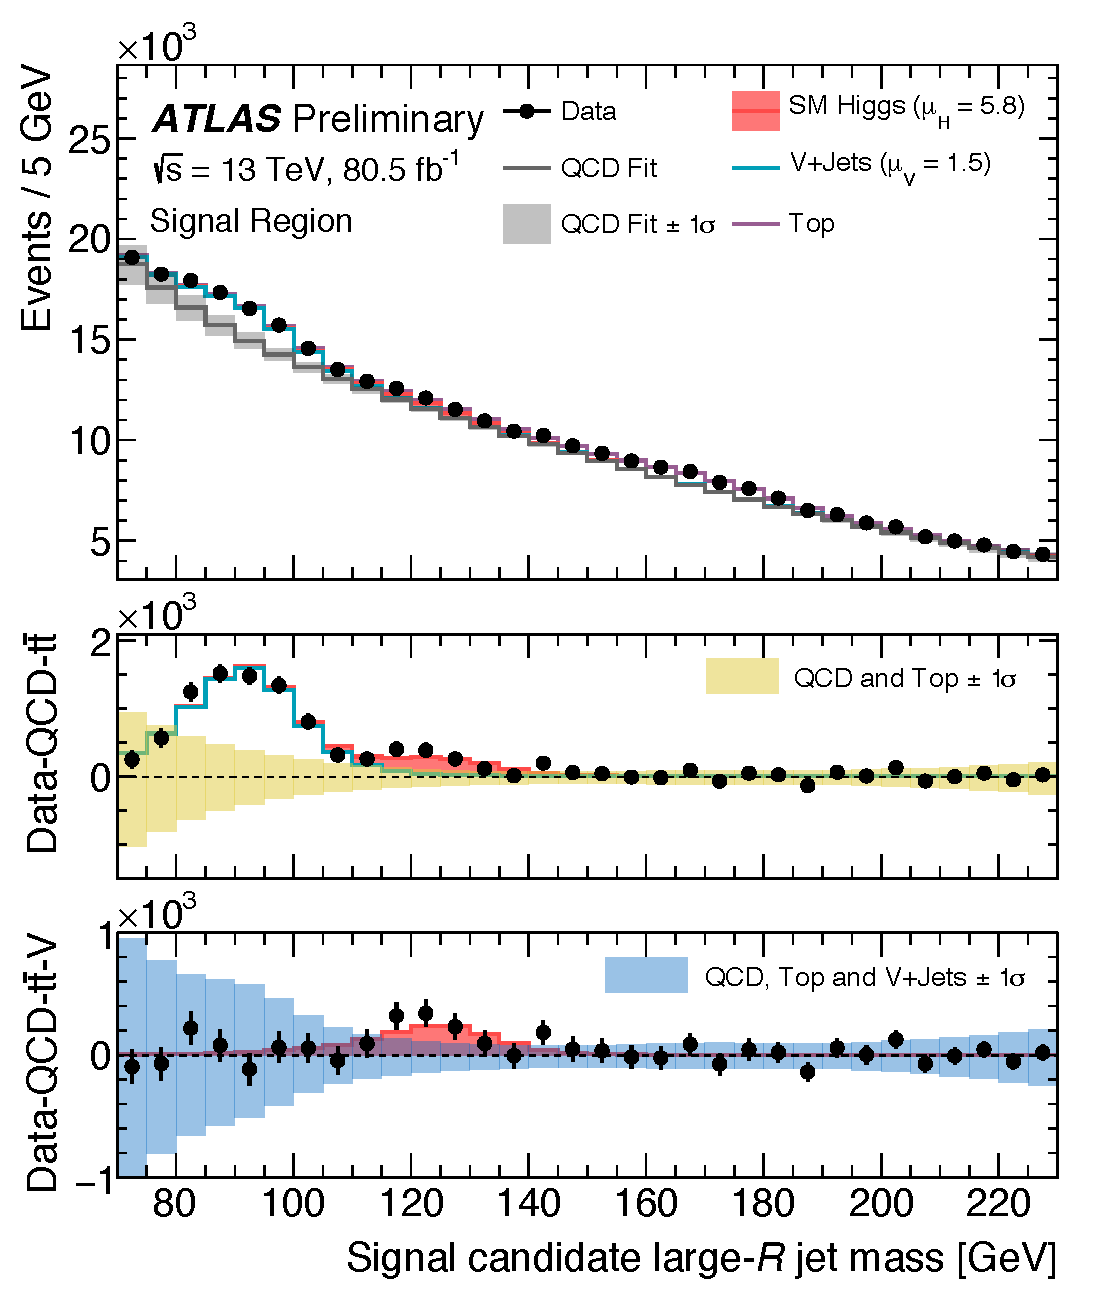
\includegraphics[width=\linewidth]{figures/results/money_plot}
\caption{ 
The top panel shows the post-fit comparison of the signal candidate large-$R$
jet mass distribution for the combined SM Higgs boson, $V$ + jets, $t\bar{t}$
and QCD model to the observed data \cite{ATLAS-CONF-2018-052}.  The middle
panel gives the ratio of the post-fit model and the data with the QCD and
$t\bar{t}$ components subtracted, highlighting the large resonance from $V$ +
jets.  The bottom panel gives the ratio of the post-fit model and the data with
the QCD, $V$ + jets, and $t\bar{t}$ components subtracted, highlighting a
slight excess of events near $m_{J} = 125~\GeV$.}
\label{sec:results:money_plot}
\end{figure}


\section{Observation of Boosted $V \rightarrow b\bar{b}$} \label{sec:results:v_jets}

The observed signal strength for the $V$ + jets process is:

$$ \mu_{V} = 1.5 \pm 0.22~\mathrm{(stat.)}^{+0.29}_{-0.25}~\mathrm{(syst.)} \pm 0.18~\mathrm{(th.)}\,, $$

corresponding to an observed significance of $5\sigma$ with an expected
significance of $4.8\sigma$ \Cite{Feickert:HiggsCouplings2018}.  This
measurement represents the first direct observation of boosted vector bosons
decaying to bottom quark pairs in ATLAS for $s = \sqrt{13}~\TeV$.

\section{Measurement of Boosted $H \rightarrow b\bar{b}$} \label{sec:results:procedure}

For the $H \rightarrow b\bar{b}$ process, the observed signal strength is:
%
$$ \mu_{H} = 5.8 \pm 3.1~\mathrm{(stat.)} \pm 1.9~\mathrm{(syst.)} \pm 1.7~\mathrm{(th.)}\,. $$
%
Given the uncertainties this result is consistent with the background-only
hypothesis at $1.6\sigma$ with an expected sensitivity of $0.28\sigma$
\cite{Feickert:HiggsCouplings2018}.  This constitutes a measurement of the
boosted Higgs decaying to a bottom quark pair but not a direct observation. The
result of the combined fit of the $V$ + jets and $H \rightarrow b\bar{b}$
signal models shows agreement with the Standard Model prediction of $\mu_{H} =
\mu_{V} = 1$ as seen in \Cref{sec:results:contour}.
%
\begin{figure}
\centering
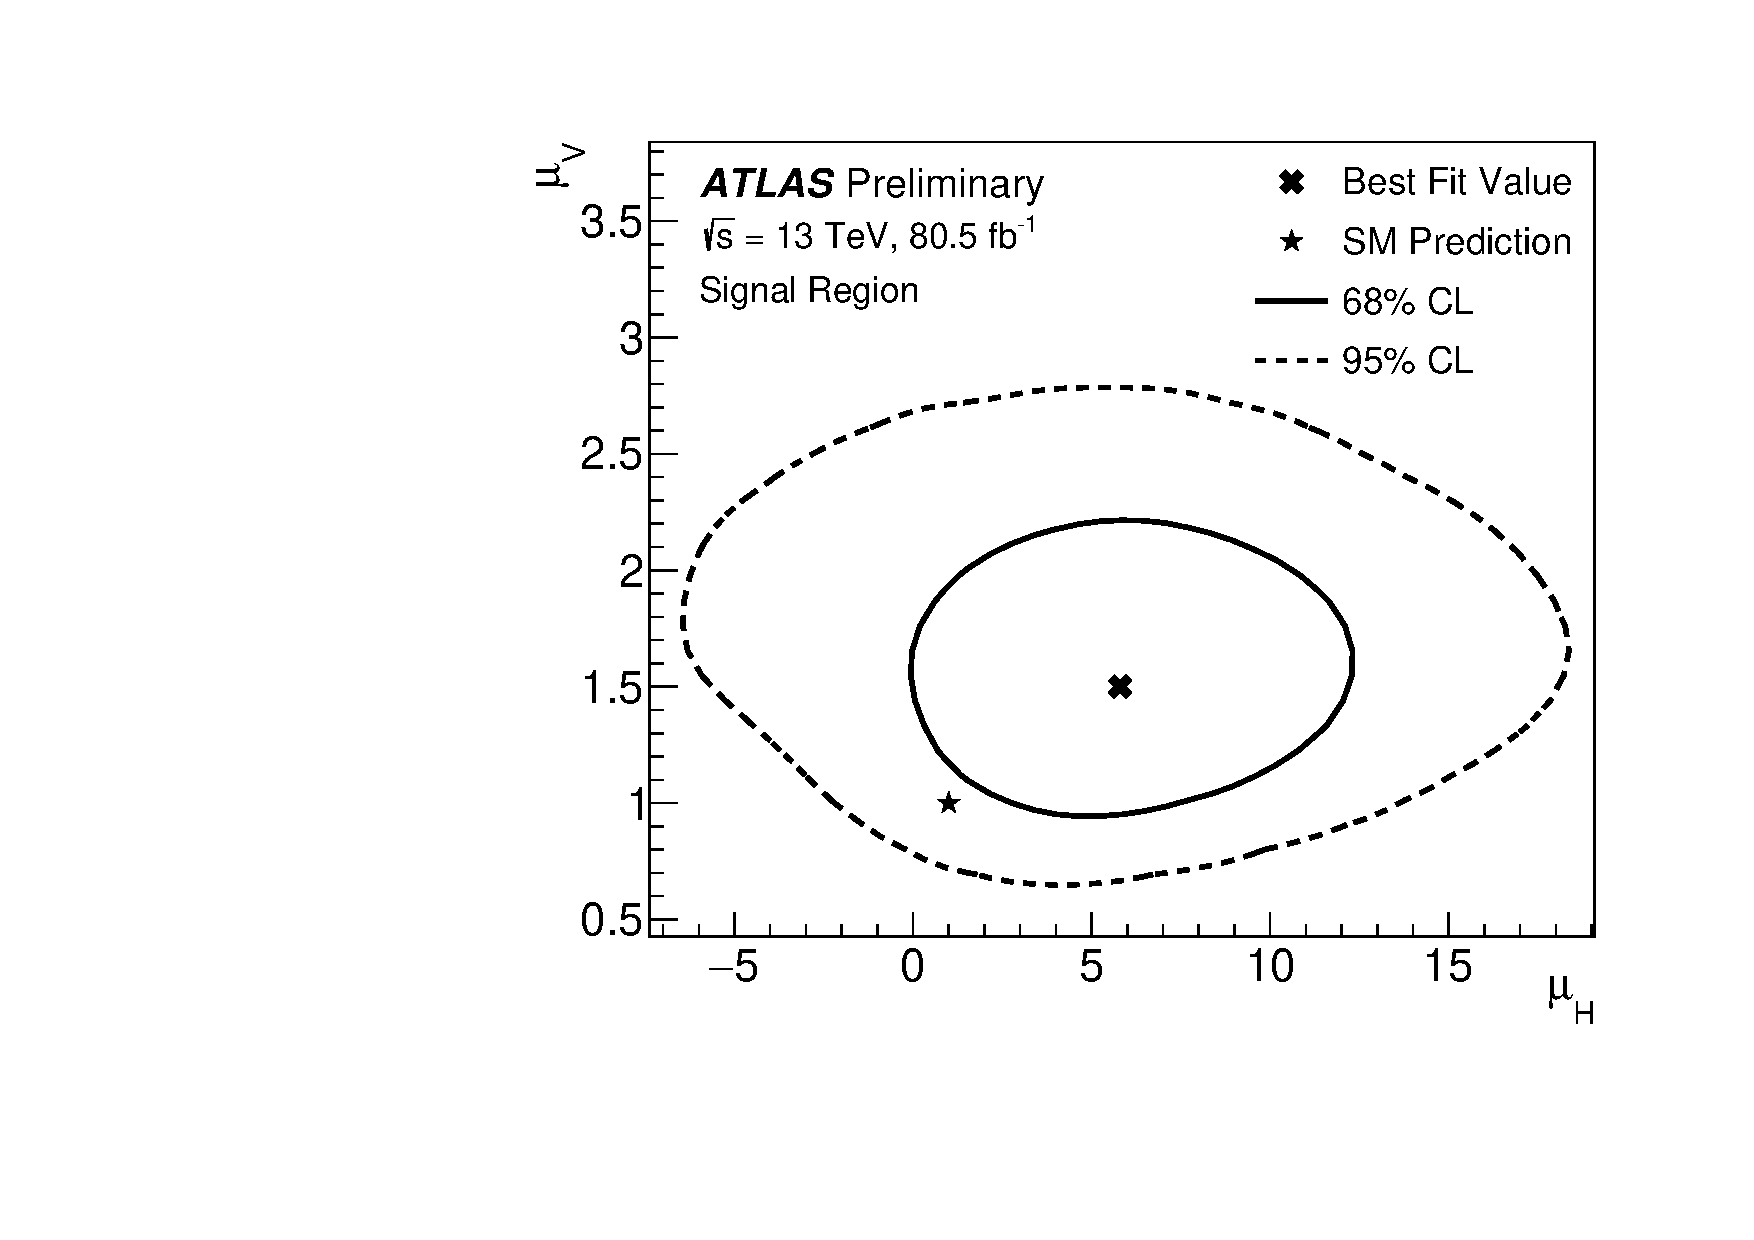
\includegraphics[width=.6\linewidth]{figures/results/contour}
\caption{\cite{ATLAS-CONF-2018-052}
Combined marginalized posterior distributions of $\mu_{H}$ and $\mu_{V}$ in the
Signal Region.  It is seen that the best-fit values for the signal processes
lie within the 68\% Credibility Level ($2\sigma$) of the Standard Model
prediction.}
\label{sec:results:contour}
\end{figure}

